\documentclass{esannV2}
\usepackage{amsmath,amssymb,graphicx,booktabs,microtype,lmodern}
\usepackage[T1]{fontenc}

\title{Which Model Changes Can Counterfactual Explanations See?\\A Ground-Truth Benchmark}
\author{[author names and affiliation withheld for review]}

\begin{document}
\maketitle

\begin{abstract}
Counterfactual methods are used to explain how a classifier changed after an update, but without ground truth one cannot tell which method explains which kind of change. We inject known changes into classifiers on rendered images with exact factors (a spurious shortcut, a shifted threshold, a subgroup label flip) next to null updates, and compare counterfactual differencing, gradient differences, importance differences, disagreement search and differential counterfactuals ($\Delta$-CE), minimal inputs on which exactly one model changes its decision by a margin. No family wins everywhere, and a pre-registered hypothesis in favour of $\Delta$-CE was rejected. Two findings were confirmed on a fresh test set: gradient differences are nearly blind to a shifted threshold (Recovery 0.10 vs.\ 0.41, difference 95\% CI [0.27, 0.35]), and margin witnesses abstain on null updates, where counterfactual differencing attributes a change to about 99\% of points. A linear analysis separating rotation from offset of the decision boundary explains the threshold result but not the shortcut result.
\end{abstract}

\section{Introduction}

Deployed classifiers are updated routinely, and an update that improves accuracy can still change individual decisions in unwanted ways [11]. Explaining \emph{how} the decisions of $f_{new}$ differ from those of $f_{old}$ is therefore a natural goal of explainable AI under distributional change [3, 12]. Artelt et al.\ [1, 2] compare a counterfactual [8] of the same input under each model, or approximate this by a difference of gradients; Muschalik et al.\ [4] compare feature importances; disagreement search [5, 6, 7] looks for inputs on which two models disagree. These families assume different things about \emph{what} changed (a direction of the weights, a boundary, a region of disagreement), and without ground truth these assumptions go unchecked.

We ask which kind of change each family can see. We inject known changes into classifiers trained on rendered images with exact generating factors and measure which factor each method attributes the change to. We also include \emph{differential counterfactuals} ($\Delta$-CE): the closest input on the data manifold at which only $f_{new}$ changes its decision while $f_{old}$ keeps it, both by a margin $\kappa$. $\Delta$-CE anchors disagreement search [5, 6] at a query; unlike robust counterfactuals [9, 10], which seek a point valid for both models, it seeks one valid for exactly one, and the margin makes it return nothing when two models differ only by jitter.

\textbf{Contributions.} (i) A benchmark with exact ground truth for explaining model updates: five rendered factors, three injected changes and two null updates (17 model pairs), with code and protocol. (ii) A comparison of five explanation families under a protocol fixed before the test data were used, reporting a rejected pre-registered hypothesis, a failed prediction and two confirmed findings. (iii) A linear analysis that separates a rotation of the decision boundary from a shift of its offset, with basic results for the margin witness.

\section{Differential counterfactuals and what each family sees}

Let $D:\mathcal Z\to\mathcal X$ map a search space onto the data manifold (here an exact renderer from factor space $\mathcal Z=[0,1]^5$). For class $y$ the margin is $m(z)=f_y(D(z))-f_{1-y}(D(z))$; $m_o,m_n$ belong to $f_{old},f_{new}$, and $h=m_n-m_o$. A query $z_0$ is valid if $m_o(z_0)\ge\kappa$ and $m_n(z_0)\ge\kappa$.

\textbf{Definition 1.} With $\mathcal F^N_\kappa=\{z: m_n(z)\le-\kappa,\ m_o(z)\ge\kappa\}$, a $\Delta$-CE of $z_0$ is $z^\star\in\arg\min_{z\in\mathcal F^N_\kappa}\|z-z_0\|$ if $\|z^\star-z_0\|\le r$, and NOT\_FOUND otherwise; swapping the models gives type O. Each $z\in\mathcal F^N_\kappa$ is a \emph{witness}: two forward passes verify that the models decide differently, both decisively, which a difference of two counterfactuals does not.

\textbf{Lemma 1.} Every witness has $h(z)\le-\kappa-m_o(z)\le-2\kappa$. Hence models whose margins differ by less than $2\kappa$ everywhere have no witness, and if $h$ is $L_h$-Lipschitz no witness lies within $(h(z_0)+2\kappa)/L_h$ of $z_0$. For deep networks $L_h$ is unknown, so this motivates the design rather than certifying it.

\textbf{Linear case.} For linear margins with independent $w_o,w_n$ the witness is unique: the ordinary counterfactual of $f_{new}$ or the minimum-norm point with both constraints active. Write $\hat w_n=\cos\theta\,\hat w_o+\sin\theta\,v$ with $v\perp\hat w_o$, and let $d_n,d_o$ be the distances from $z_0$ to $\{m_n=-\kappa\}$ and $\{m_o=\kappa\}$. The gradient difference of [1] is $-(\hat w_n-\hat w_o)$, counterfactual differencing is $u_n-u_o$, the witness is $u^\star$.

\textbf{Proposition 2.} (a) \emph{Offset} ($\theta=0$): the gradient difference is $0$; counterfactual differencing is a multiple of $\hat w_o$; a witness exists iff $d_n\le d_o$ and equals $-d_n\hat w_o$. (b) \emph{Rotation} ($0<\theta<\pi/2$): the gradient difference has components in ratio $\tan(\theta/2)<1$ along $(\hat w_o,v)$, i.e.\ mainly along the new dependence $v$; the witness has $|u^\star\!\cdot\hat w_o|=\min\{d_n\cos\theta,d_o\}$ and, for $\theta\le\pi/4$, is dominated by $v$ only if $d_o(\sin\theta+\cos\theta)<d_n$. After projecting out $\hat w_o$ all three coincide, as in Theorem 1 of [1].

Proofs are at [link]; a numerical check on linear models agrees with the solver on distances to within $10^{-3}$, although a stricter pre-declared vector criterion failed at $p=5$. In words, gradient differences see a \emph{rotation} of the boundary and are blind to a shift of its \emph{offset}; counterfactual differencing and witnesses see the offset, and witnesses abstain when the shift is below $2\kappa$. This analysis was formulated after the main experiment.

\section{Benchmark and protocol}

\textbf{Data and models.} Images are $32\times32$ ellipses rendered from five independent factors in $[0,1]$: aspect (task factor), size, colour, background and horizontal position; labels are $y=\mathbb 1[\text{aspect}>0.5]$ with 5\% noise. The renderer is exact, so the factor change of any explanation is read without a learned oracle. $f_{old}$ is a small CNN (five seeds); $f_{new}$ is $f_{old}$ fine-tuned on 10\,000 samples from one of five conditions (Table~\ref{tab:changes}). A pair enters only if its change is visible in decisions on validation data (pre-declared thresholds on decision flips per factor; null pairs need decisive disagreement $\le0.02$); all 17 qualified.

\begin{table}[t]
\caption{Injected changes; $k^\star$ is the ground-truth factor.}
\label{tab:changes}
\centering\footnotesize
\begin{tabular}{lllc}
\toprule
Code & Adaptation data & $k^\star$ & Pairs\\
\midrule
T1 shortcut & colour correlated with label (0.99), near the boundary & colour & 3\\
T3 subgroup & labels flipped for size $>0.75$ & size & 3\\
T4 threshold & $y=\mathbb 1[\text{aspect}>0.6]$ & aspect & 3\\
N0 / N1 null & resample / size $\sim U[0.5,1]$, same rule & --- & 5 / 3\\
\bottomrule
\end{tabular}
\end{table}

\textbf{Metrics and methods.} Per pair we use $N=300$ valid test points. $\mathrm{Recovery@}r$ is the share of points with a valid explanation within the budget whose largest factor change is $k^\star$ (NOT\_FOUND and ties count 0). All counterfactual methods share one solver (Adam with a decaying penalty, then SLSQP on the constrained problem), the same points and the same budget $r=0.54$, set once on validation. We compare $\Delta$-CE ($\kappa=0.5$); \textbf{B1} counterfactual differencing [1] and a deterministic variant \textbf{B1-det}; \textbf{B3} gradient difference [1]; \textbf{B4} permutation-importance difference [4]; \textbf{B5} DIG-style line search [5]; \textbf{A1} DeepXplore-style search without proximity [6]; \textbf{A2} the ordinary counterfactual of $f_{new}$ alone.

\textbf{Protocol.} All choices were fixed before the test split was used once. \emph{Pre-registered:} H2a ($\Delta$-CE beats B3 on T3; paired bootstrap stratified by pair, 95\% CI, all three seeds) and a tie on T1 and T4 ($|\Delta|\le0.10$). \emph{Confirmatory:} readings formed after the results, tested on a new test set with the same models (C1--C3, Holm-corrected). \emph{Descriptive:} the rest. A second tier on coloured digits and a label-shift update failed pre-declared qualification and were stopped.

\section{Results}

\begin{table}[t]
\caption{Recovery@$r$ (found-rate) on the locked test split, mean over three pairs; all 95\% bootstrap CIs within $\pm0.035$. Last row: found-rate on the 8 null pairs.}
\label{tab:results}
\centering\small
\resizebox{\linewidth}{!}{%
\begin{tabular}{lcccccccc}
\toprule
 & $\Delta$-CE & B1 & B1-det & B3 & B4 & B5 & A1 & A2\\
\midrule
T1 & 0.38 (0.84) & 0.54 (0.93) & 0.54 (0.93) & \textbf{0.91} (1.0) & 0.00 & 0.02 (0.08) & 0.35 (0.63) & 0.07 (0.93)\\
T3 & 0.53 (0.81) & 0.32 (1.0) & 0.32 (0.99) & \textbf{0.62} (1.0) & 0.00 & 0.06 (0.10) & 0.29 (0.58) & 0.30 (1.0)\\
T4 & 0.47 (0.47) & 0.77 (0.90) & 0.76 (0.90) & 0.07 (1.0) & \textbf{1.00} & 0.07 (0.08) & 0.31 (0.40) & 0.90 (0.90)\\
Null & \textbf{0.000} & 0.995 & 0.994 & 1.0 & 1.0 & 0.000 & 0.000 & 0.996\\
\bottomrule
\end{tabular}}
\end{table}

\textbf{Pre-registered.} H2a is \emph{rejected}: on T3, Recovery($\Delta$-CE) $-$ Recovery(B3) $=-0.091$, 95\% CI $[-0.133,-0.050]$, negative in all seeds. $\Delta$-CE beats B1 (+0.21, descriptive) and B5 (+0.47, CI [0.43, 0.50]), which rarely reaches the disagreement region (found-rate $\le0.11$); we make no solver claim from one benchmark. The predicted tie also fails: all four comparisons exceed 0.10 (T1 vs.\ B3 $-0.53$, vs.\ B1-det $-0.17$; T4 vs.\ B3 $+0.40$, vs.\ B1-det $-0.29$). B1 and B1-det agree within 0.01 everywhere.

\textbf{Null updates.} On all eight null pairs $\Delta$-CE returns no witness, while B1 attributes a change to 99.5\% of points. With $\kappa=0$ witnesses reappear (found-rate 0.80 on N0, 0.89 on N1), as Lemma 1 predicts. All methods separate drift from null pairs at the pair level (AUROC 1.0), so the difference lies in what each says about a null update.

\textbf{Confirmed on a new test set.} \emph{C1 (offset blindness), confirmed:} on T4, Recovery($\Delta$-CE) $-$ Recovery(B3) $=+0.31$, 95\% CI $[0.27,0.35]$, $p_{Holm}=2\cdot10^{-4}$, positive in all seeds ($\Delta$-CE 0.41, B3 0.10, B1-det 0.76), the CNN counterpart of Proposition 2(a). Its content is the failure of B3: on an offset change the changed factor is the task factor, so even A2 recovers it (0.90). \emph{C2 (abstention), confirmed:} no witness on any null pair; B1 attributes a change to 99.1\% (N0) and 99.8\% (N1) of points. \emph{C3 (rotation after projection), not confirmed:} Proposition 2(b) predicts that $\Delta$-CE and B3 coincide on T1 once $\hat w_o$ is projected out; they do not (0.64 vs.\ 0.95, difference $-0.30$, 90\% CI $[-0.33,-0.28]$). The T1 outcome remains unexplained.

\begin{figure}[t]
\centering
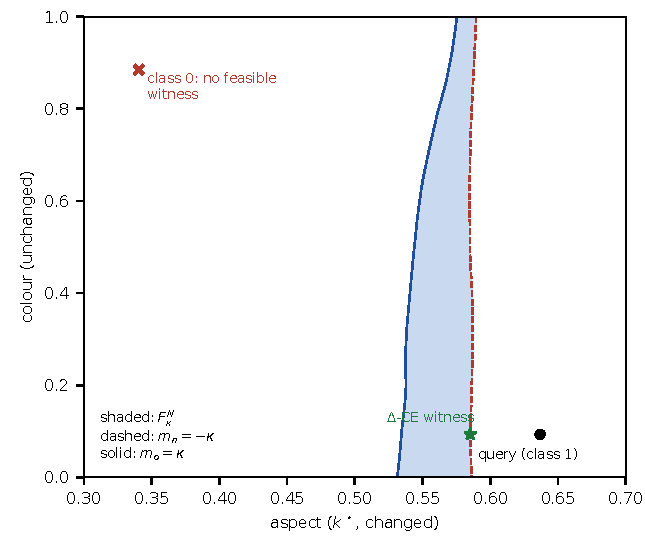
\includegraphics[width=0.62\linewidth,trim=0 70 0 0,clip]{figures/fig1_t4.pdf}
\caption{T4 (one pair) in the (aspect, colour) plane, other factors at the query's values: boundaries of $f_{old}$ (solid) and $f_{new}$ (dashed), witness region $\mathcal F^N_\kappa$ (shaded), a class-1 query and its witness, and a class-0 point with no feasible witness. Illustrative, not a result.}
\label{fig:t4}
\end{figure}

\textbf{Where witnesses exist (descriptive).} On T4 a witness is found for every class-1 point and for no class-0 point, in all pairs and on both test sets (e.g.\ 136/136 vs.\ 0/164); class-0 failures are infeasible, not over budget (Fig.~\ref{fig:t4}). This is what Proposition 2(a) implies for an offset that lowers the margin of one class, and the class-wise statement was written before the split was computed. It is what a witness adds on T4 beyond the direction: the side of the boundary on which decisions flipped. On T1 and T3, 16--17\% of points have a witness beyond the budget; halving the budget halves the found-rate.

\section{Discussion and limitations}

Which family explains a model change depends on the kind of change. Gradient differences recover a change of direction (T1) and are nearly blind to a change of offset (T4). Counterfactual differencing cannot say that nothing changed. Margin witnesses are the only family that abstains on null updates and returns checkable inputs, but they are limited by feasibility and budget and lose on the subgroup change. A reading not tested as a procedure is to use witnesses to decide \emph{whether} decisions changed near a query and other families to describe \emph{how}.

\textbf{Limitations.} (1) The data are synthetic; a tier on coloured digits failed qualification because fine-tuning a strong model no longer produced the injected changes. (2) Proposition 2(a) implies that the update optimal under label shift, a pure offset [13], is invisible to gradient differences, but our label-shift update created no decisive disagreements, so this remains open. (3) T1 is unexplained (C3). (4) Witnesses see only decision changes on the manifold within the budget, with no certificate for deep networks. (5) C1--C3 were formed after the main experiment. (6) On offset changes Recovery rewards any explanation that follows $f_{new}$ (A2: 0.90), so it measures blindness rather than sensitivity; a metric that scores \emph{where} an explanation is returned is needed. The protocol went through eight logged amendments and two pre-declared stopping rules; history, proofs and code are at [link].

\begin{footnotesize}
\begin{thebibliography}{13}
\bibitem{r1} A. Artelt, F. Hinder, V. Vaquet, R. Feldhans, B. Hammer. Contrastive explanations for explaining model adaptations. arXiv:2104.02459, 2021.
\bibitem{r2} A. Artelt et al. Contrasting explanations for understanding and regularizing model adaptations. \emph{Neural Processing Letters}, 2022. [verify]
\bibitem{r4} B. Hammer, E. H\"ullermeier. Interpretable machine learning: on the problem of explaining model change. 2021. [verify venue]
\bibitem{r5} M. Muschalik, F. Fumagalli, B. Hammer, E. H\"ullermeier. Agnostic explanation of model change based on feature importance. \emph{KI -- K\"unstliche Intelligenz}, 2022.
\bibitem{r6} X. Renard, T. Laugel, M. Detyniecki. Understanding prediction discrepancies in machine learning classifiers. arXiv:2104.05467, 2021.
\bibitem{r7} K. Pei, Y. Cao, J. Yang, S. Jana. DeepXplore: automated whitebox testing of deep learning systems. \emph{SOSP}, 2017.
\bibitem{r8} M. Augustin et al. DiG-IN: diffusion guidance for investigating networks. \emph{CVPR}, 2024.
\bibitem{r9} S. Wachter, B. Mittelstadt, C. Russell. Counterfactual explanations without opening the black box. \emph{Harvard J. Law \& Technology}, 2017.
\bibitem{r10} F. Hamman et al. Robust counterfactual explanations for neural networks with probabilistic guarantees. \emph{ICML}, 2023.
\bibitem{r11} M. Pawelczyk, K. Broelemann, G. Kasneci. On counterfactual explanations under predictive multiplicity. \emph{UAI}, 2020.
\bibitem{r12} S. Yan, Y. Xiong, K. Kundu, S. Yang, S. Deng, M. Wang, W. Xia, S. Soatto. Positive-congruent training: towards regression-free model updates. \emph{CVPR}, 2021. [verify venue]
\bibitem{r13} M. Kaden, B. Paassen, B. Hammer, R. Schubert, T. Villmann. Reliable counterfactuals for machine learning models --- current aspects and perspectives. \emph{ESANN}, 2026. [verify]
\bibitem{r14} M. Saerens, P. Latinne, C. Decaestecker. Adjusting the outputs of a classifier to new a priori probabilities: a simple procedure. \emph{Neural Computation} 14(1):21--41, 2002.
\end{thebibliography}
\end{footnotesize}

\end{document}
